\documentclass[11pt]{article}
\usepackage{amsmath,amssymb,amsthm}
\usepackage{graphicx}
\usepackage[margin=1in]{geometry}
\usepackage{fancyhdr}
\usepackage{float}
\setlength{\parindent}{0pt}
\setlength{\parskip}{5pt plus 1pt}
\setlength{\headheight}{13.6pt}
\newcommand\question[2]{\vspace{.25in}\hrule\textbf{#1: #2}\vspace{.5em}\hrule\vspace{.10in}}
\renewcommand\part[1]{\vspace{.10in}\textbf{(#1)}}
\newcommand\algorithm{\vspace{.10in}\textbf{Algorithm: }}
\newcommand\result{\vspace{.10in}\textbf{Result: }}
\pagestyle{fancyplain}
\lhead{\textbf{\NAME\ (\ANDREWID)}}
\chead{\textbf{Assignment\HWNUM}}
\rhead{STAT3006: Statistical Computing}
\begin{document}\raggedright
%Section A==============Change the values below to match your information==================
\newcommand\NAME{ZHANG Xinfang}  % your name
\newcommand\ANDREWID{1155141566}     % your student id
\newcommand\HWNUM{1}              % the homework number
%Section B==============Put your answers to the questions below here=======================

\question{1}{The Bisection Method (25\%)} 
For function $f(x) = x^3 + 6x^2 + \pi x - 12$, the derivative is $f'(x) = 3x^2 + 12x + \pi$. The we can calculate that 
zeros of the derivative are $\frac{-12 - \sqrt{12(12-\pi)}}{6}$ and $\frac{-12 + \sqrt{12(12-\pi)}}{6}$.

$f(\frac{-12 - \sqrt{12(12-\pi)}}{6}) = 7.864841$ and $f(\frac{-12 + \sqrt{12(12-\pi)}}{6}) = -12.43121$
Hence, the function $f$ has totally 3 zeros.

\algorithm{Bisection Method in the R file.}

\result{Zeros: -4.837944, -2.259727, and 1.097664.}

\question{2}{Poisson Regression - Newton's Method (25\%)}

\part{1} Since $y_i \sim Poisson(\lambda_i)$ and $log(\lambda_i) = \alpha + \beta x_i + \gamma x_i^2$, we can get the Likelihhod function:

\begin{align*}
    L(\alpha, \beta, \gamma|\mathbf{x}, \mathbf{y}) = \prod_{i=1}^{n} \frac{\lambda_i^{y_i} e^{-\lambda_i}}{y_i !} = \prod_{i=1}^{n} \frac{e^{(\alpha + \beta x_i + \gamma x_i^2)y_i} e^{-e^{\alpha + \beta x_i + \gamma x_i^2}}}{y_i !}
\end{align*}

\part{2} The log-Likelihood function is 
\begin{align*}
    l(\alpha, \beta, \gamma|\mathbf{x}, \mathbf{y}) = \sum_{i=1}^{n} (\alpha + \beta x_i + \gamma x_i^2)y_i - e^{\alpha + \beta x_i + \gamma x_i^2} - \log y_i !  
\end{align*}
Then we have:
\begin{align*}
    \frac{\partial l(\alpha, \beta, \gamma|\mathbf{x}, \mathbf{y})}{\partial \alpha}\bigg\rvert_{\hat{\alpha}} &= \sum_{i=1}^{n} [y_i - e^{\alpha + \beta x_i + \gamma x_i^2}]\bigg\rvert_{\hat{\alpha}} = 0\\
    \frac{\partial l(\alpha, \beta, \gamma|\mathbf{x}, \mathbf{y})}{\partial \beta}\bigg\rvert_{\hat{\beta}} &= \sum_{i=1}^{n} [x_iy_i - x_ie^{\alpha + \beta x_i + \gamma x_i^2}]\bigg\rvert_{\hat{\beta}} = 0\\
    \frac{\partial l(\alpha, \beta, \gamma|\mathbf{x}, \mathbf{y})}{\partial \gamma}\bigg\rvert_{\hat{\gamma}} &= \sum_{i=1}^{n} [x_i^2y_i - x_i^2e^{\alpha + \beta x_i + \gamma x_i^2}]\bigg\rvert_{\hat{\gamma}} = 0\\
\end{align*}
Let $\mathbf{F}(\mathbf{x}) = \begin{pmatrix}
    \frac{\partial l(\alpha, \beta, \gamma|\mathbf{x}, \mathbf{y})}{\partial \alpha}\\\frac{\partial l(\alpha, \beta, \gamma|\mathbf{x}, \mathbf{y})}{\partial \beta}\\\frac{\partial l(\alpha, \beta, \gamma|\mathbf{x}, \mathbf{y})}{\partial \gamma}
\end{pmatrix}$, then $\mathbf{F'}(\mathbf{x}) = \begin{pmatrix}
    \frac{\partial^2 l(\alpha, \beta, \gamma|\mathbf{x}, \mathbf{y})}{\partial \alpha^2} && \frac{\partial^2 l(\alpha, \beta, \gamma|\mathbf{x}, \mathbf{y})}{\partial \beta \partial \alpha} && \frac{\partial^2 l(\alpha, \beta, \gamma|\mathbf{x}, \mathbf{y})}{\partial \gamma \partial \alpha}\\
    \frac{\partial^2 l(\alpha, \beta, \gamma|\mathbf{x}, \mathbf{y})}{\partial \alpha \partial \beta} && \frac{\partial^2 l(\alpha, \beta, \gamma|\mathbf{x}, \mathbf{y})}{\partial \beta^2} && \frac{\partial^2 l(\alpha, \beta, \gamma|\mathbf{x}, \mathbf{y})}{\partial \gamma \partial \beta}\\
    \frac{\partial^2 l(\alpha, \beta, \gamma|\mathbf{x}, \mathbf{y})}{\partial \alpha \partial \gamma} && \frac{\partial^2 l(\alpha, \beta, \gamma|\mathbf{x}, \mathbf{y})}{\partial \beta \partial \gamma} && \frac{\partial^2 l(\alpha, \beta, \gamma|\mathbf{x}, \mathbf{y})}{\partial \gamma^2}
\end{pmatrix}$, in which 
\begin{flalign*}
    \frac{\partial^2 l(\alpha, \beta, \gamma|\mathbf{x}, \mathbf{y})}{\partial \alpha^2} &= \sum_{i=1}^{n} -e^{\alpha + \beta x_i + \gamma x_i^2}\\
    \frac{\partial^2 l(\alpha, \beta, \gamma|\mathbf{x}, \mathbf{y})}{\partial \alpha \partial \beta} &= \frac{\partial^2 l(\alpha, \beta, \gamma|\mathbf{x}, \mathbf{y})}{\partial \beta \partial \alpha} = \sum_{i=1}^{n} -x_ie^{\alpha + \beta x_i + \gamma x_i^2}\\
    \frac{\partial^2 l(\alpha, \beta, \gamma|\mathbf{x}, \mathbf{y})}{\partial \alpha \partial \gamma} &= \frac{\partial^2 l(\alpha, \beta, \gamma|\mathbf{x}, \mathbf{y})}{\partial \gamma \partial \alpha} = \sum_{i=1}^{n} -x_i^2e^{\alpha + \beta x_i + \gamma x_i^2}\\
    \frac{\partial^2 l(\alpha, \beta, \gamma|\mathbf{x}, \mathbf{y})}{\partial \beta^2} &= \sum_{i=1}^{n} -x_i^2e^{\alpha + \beta x_i + \gamma x_i^2}\\
    \frac{\partial^2 l(\alpha, \beta, \gamma|\mathbf{x}, \mathbf{y})}{\partial \beta \partial \gamma} &= \frac{\partial^2 l(\alpha, \beta, \gamma|\mathbf{x}, \mathbf{y})}{\partial \gamma \partial \beta} = \sum_{i=1}^{n} -x_i^3e^{\alpha + \beta x_i + \gamma x_i^2}\\
    \frac{\partial^2 l(\alpha, \beta, \gamma|\mathbf{x}, \mathbf{y})}{\partial \gamma^2} &= \sum_{i=1}^{n} -x_i^4e^{\alpha + \beta x_i + \gamma x_i^2}
\end{flalign*}
Therefore, by Newton's Methhod, given initial guess $\alpha^{(0)}$, $\beta^{(0)}$, and $\gamma^{(0)}$, for each iteration: 
\begin{align*}
    \begin{pmatrix} \alpha^{(n)} \\ \beta^{(n)} \\ \gamma^{(n)} \end{pmatrix} = \begin{pmatrix} \alpha^{(n-1)} \\ \beta^{(n-1)} \\ \gamma^{(n-1)} \end{pmatrix} - \mathbf{F'}[(\mathbf{x})]^{-1}\mathbf{F}(\mathbf{x}).
\end{align*}
Hence, for the algorithm: $\mathbf{x^{(n)}} = \begin{pmatrix} \alpha^{(n)} \\ \beta^{(n)} \\ \gamma^{(n)} \end{pmatrix}$,

STEP 1: Solve $\mathbf{F'}(\mathbf{x^{(n)}}) \mathbf{\triangle x^{(n)}} = - \mathbf{F}(\mathbf{x^{(n)}})$;

STEP 2: Update by $\mathbf{x^{(n+1)}} = \mathbf{x^{(n)}} + \mathbf{\triangle x^{(n)}}$.

\part{3} 

\algorithm{Newton's Method code in the R file.}

\result{$\alpha = 1.503533$, $\beta = 1.052351$, and $\gamma = 1.957396$.}

\question{3}{Logistic Regression - Newton's Method (20\%)}

\part{1} Since $y_i \sim Bernoulli(p_i)$ and $logit(p_i) = \alpha + \beta x_i$, we can know that $f(y_i, p_i) = p_i^{y_i}(1-p_i)^{1-y_i}$,
and $p_i = \frac{e^{\alpha + \beta x_i}}{1 + e^{\alpha + \beta x_i}}$. Then we can get the following Likelihood function:
\begin{flalign*}
    L(\alpha, \beta | \mathbf{x}, \mathbf{y}) &= \prod_{i=1}^{n} p_i^{y_i}(1-p_i)^{1-y_i}\\
                                              &= \prod_{i=1}^{n} ({\frac{e^{\alpha + \beta x_i}}{1 + e^{\alpha + \beta x_i}}})^{y_i}(1-{\frac{e^{\alpha + \beta x_i}}{1 + e^{\alpha + \beta x_i}}})^{1-y_i}
\end{flalign*}
\part{2} The log-Likelihood function is 
\begin{flalign*}
    l(\alpha, \beta | \mathbf{x}, \mathbf{y}) &= \sum_{i=1}^n y_i (\alpha + \beta x_i - \log(1+e^{\alpha + \beta x_i})) + (1 - y_i)\log(\frac{1}{1 + e^{\alpha + \beta x_i}})\\
                                              &= \sum_{i=1}^n \alpha x_i + \beta x_i y_i - \log (1+e^{\alpha + \beta x_i})
\end{flalign*}
Then we have:
\begin{flalign*}
    \frac{\partial l(\alpha, \beta|\mathbf{x}, \mathbf{y})}{\partial \alpha}\bigg\rvert_{\hat{\alpha}} &= \sum_{i=1}^{n} [y_i - \frac{e^{\alpha + \beta x_i}}{1 + e^{\alpha + \beta x_i}}] \bigg\rvert_{\hat{\alpha}} = 0\\
    \frac{\partial l(\alpha, \beta|\mathbf{x}, \mathbf{y})}{\partial \beta}\bigg\rvert_{\hat{\beta}} &= \sum_{i=1}^{n} [x_i y_i - \frac{x_i e^{\alpha + \beta x_i}}{1 + e^{\alpha + \beta x_i}}] \bigg\rvert_{\hat{\beta}} = 0
\end{flalign*}
Let $\mathbf{F}(\mathbf{x}) = \begin{pmatrix}
    \frac{\partial l(\alpha, \beta|\mathbf{x}, \mathbf{y})}{\partial \alpha}\\\frac{\partial l(\alpha, \beta|\mathbf{x}, \mathbf{y})}{\partial \beta}
\end{pmatrix}$, then $\mathbf{F'}(\mathbf{x}) = \begin{pmatrix}
    \frac{\partial^2 l(\alpha, \beta|\mathbf{x}, \mathbf{y})}{\partial \alpha^2} && \frac{\partial^2 l(\alpha, \beta|\mathbf{x}, \mathbf{y})}{\partial \beta \partial \alpha} \\
    \frac{\partial^2 l(\alpha, \beta|\mathbf{x}, \mathbf{y})}{\partial \alpha \partial \beta} && \frac{\partial^2 l(\alpha, \beta|\mathbf{x}, \mathbf{y})}{\partial \beta^2}
\end{pmatrix}$, in which 
\begin{flalign*}
    \frac{\partial^2 l(\alpha, \beta|\mathbf{x}, \mathbf{y})}{\partial \alpha^2} &= -\frac{e^{\alpha + \beta x_i}}{(1+e^{\alpha + \beta x_i})^2}\\
    \frac{\partial^2 l(\alpha, \beta|\mathbf{x}, \mathbf{y})}{\partial \beta \partial \alpha} &= \frac{\partial^2 l(\alpha, \beta|\mathbf{x}, \mathbf{y})}{\partial \alpha \partial \beta} = -\frac{x_i e^{\alpha + \beta x_i}}{(1+e^{\alpha + \beta x_i})^2}\\
    \frac{\partial^2 l(\alpha, \beta|\mathbf{x}, \mathbf{y})}{\partial \beta^2} &= -\frac{x_i^2 e^{\alpha + \beta x_i}}{(1+e^{\alpha + \beta x_i})^2}
\end{flalign*}
Therefore, by Newton's Methhod, given initial guess $\alpha^{(0)}$ and $\beta^{(0)}$, for each iteration: 
\begin{align*}
    \begin{pmatrix} \alpha^{(n)} \\ \beta^{(n)} \end{pmatrix} = \begin{pmatrix} \alpha^{(n-1)} \\ \beta^{(n-1)} \end{pmatrix} - \mathbf{F'}[(\mathbf{x})]^{-1}\mathbf{F}(\mathbf{x}).
\end{align*}
Hence, for the algorithm: $\mathbf{x^{(n)}} = \begin{pmatrix} \alpha^{(n)} \\ \beta^{(n)} \end{pmatrix}$,

STEP 1: Solve $\mathbf{F'}(\mathbf{x^{(n)}}) \mathbf{\triangle x^{(n)}} = - \mathbf{F}(\mathbf{x^{(n)}})$;

STEP 2: Update by $\mathbf{x^{(n+1)}} = \mathbf{x^{(n)}} + \mathbf{\triangle x^{(n)}}$.

\part{3}

\algorithm{Newton's Method code in the R file.}

\result{$\alpha = 1.564284$ and $\beta = 1.771093$.}

\question{4}{EM Algorithm (30\%)}

\part{1} Observed data: $Y_i$ for $i = 1$, $2, \dots$, $8000$; Missing data: $Z_i$ for $i = 1$, $2, \dots$, $8000$., where $Z_i = 1$, 2, or 3 for low, middle, and high income respectively.

Since $Y_i \big\rvert (Z_i=k) \sim N(\mu_k, \sigma_k^2)$, with proportion $\pi_k$ ($\pi_3 = 1 - (\pi_1 + \pi_2)$), we can formulate 

the $\mathbf{complete-data}$ $\mathbf{Likelihhod}$ $\mathbf{function}$ as:
\begin{flalign*}
    &L(\pi_1, \pi_2, \mu_1, \mu_2, \mu_3, \sigma_1, \sigma_2, \sigma_3 | \mathbf{Y}, \mathbf{Z})\\
   =&\prod_{i=1}^{n} \Biggl[\pi_1 \frac{1}{\sqrt{2\pi}\sigma_1}e^{-\frac{(y_i-\mu_1)^2}{2\sigma_1^2}}\Biggr]^{I(Z_i = 1)} \Biggl[\pi_2 \frac{1}{\sqrt{2\pi}\sigma_2}e^{-\frac{(y_i-\mu_2)^2}{2\sigma_2^2}}\Biggr]^{I(Z_i = 2)} \Biggl[(1-\pi_1-\pi_2) \frac{1}{\sqrt{2\pi}\sigma_3}e^{-\frac{(y_i-\mu_3)^2}{2\sigma_3^2}}\Biggr]^{I(Z_i = 3)}
\end{flalign*}
The observed-data Likelihhod function is:
\begin{flalign*}
    &L(\pi_1, \pi_2, \mu_1, \mu_2, \mu_3, \sigma_1, \sigma_2, \sigma_3 | \mathbf{Y})\\
   =&\prod_{i=1}^{n} \Biggl[ \biggl[\pi_1 \frac{1}{\sqrt{2\pi}\sigma_1}e^{-\frac{(y_i-\mu_1)^2}{2\sigma_1^2}}\biggr] +  \biggl[\pi_2 \frac{1}{\sqrt{2\pi}\sigma_2}e^{-\frac{(y_i-\mu_2)^2}{2\sigma_2^2}}\biggr] + \biggl[(1-\pi_1-\pi_2) \frac{1}{\sqrt{2\pi}\sigma_3}e^{-\frac{(y_i-\mu_3)^2}{2\sigma_3^2}}\biggr] \Biggr]
\end{flalign*}
\part{2} The complete-data log-Likelihhod function is:
\begin{flalign*}
    l(\pi_1, \pi_2, \mu_1, \mu_2, \mu_3, \sigma_1, \sigma_2, \sigma_3 | \mathbf{Y}, \mathbf{Z}) =\sum_{i=1}^n \Biggl[&I(Z_i = 1) \biggl[\log \pi_1 - \log \sqrt{2\pi} - \frac{1}{2}\log \sigma_1^2 - \frac{(y_i - \mu_1)^2}{2 \sigma_1^2}\biggr]\\
                                                                                                                    +&I(Z_i = 2) \biggl[\log \pi_2 - \log \sqrt{2\pi} - \frac{1}{2}\log \sigma_2^2 - \frac{(y_i - \mu_2)^2}{2 \sigma_2^2}\biggr]\\
                                                                                                                    +&I(Z_i = 3) \biggl[\log (1-\pi_1-\pi_2) - \log \sqrt{2\pi} - \frac{1}{2}\log \sigma_3^2 - \frac{(y_i - \mu_3)^2}{2 \sigma_3^2}\biggr]\Biggr]
\end{flalign*}
Then given initial guess $\pi_1^{(0)}, \pi_2^{(0)}, \mu_1^{(0)}, \mu_2^{(0)}, \mu_3^{(0)}, \sigma_1^{(0)}, \sigma_2^{(0)}, \sigma_3^{(0)}$, 
we define a $Q$ function by $Q(\Theta; \Theta^{(t)}) = E_{\mathbf{\Theta^{(t)}}} \bigl( l(\mathbf{\Theta} | \mathbf{Y}, \mathbf{Z}) | \mathbf{Y} \bigr)$:
\begin{flalign*}
    Q(\Theta; \Theta^{(t)}) &= E_{\pi_1^{(t)}, \pi_2^{(t)}, \mu_1^{(t)}, \mu_2^{(t)}, \mu_3^{(t)}, {\sigma_1^2}^{(t)}, {\sigma_2^2}^{(t)}, {\sigma_3^2}^{(t)}} \bigl( l(\pi_1, \pi_2, \mu_1, \mu_2, \mu_3, \sigma_1, \sigma_2, \sigma_3 | \mathbf{Y}, \mathbf{Z}) | \mathbf{Y} \bigr)\\
                            &= \sum_{i=1}^n \Biggl[\widehat{Z_{i1}}^{(t)} \biggl[\log \pi_1 - \log \sqrt{2\pi} - \frac{1}{2}\log \sigma_1^2 - \frac{(y_i - \mu_1)^2}{2 \sigma_1^2}\biggr]\\
                            &+ \widehat{Z_{i2}}^{(t)} \biggl[\log \pi_2 - \log \sqrt{2\pi} - \frac{1}{2}\log \sigma_2^2 - \frac{(y_i - \mu_2)^2}{2 \sigma_2^2}\biggr]\\
                            &+ \widehat{Z_{i3}}^{(t)} \biggl[\log (1-\pi_1-\pi_2) - \log \sqrt{2\pi} - \frac{1}{2}\log \sigma_3^2 - \frac{(y_i - \mu_3)^2}{2 \sigma_3^2}\biggr]\Biggr]
\end{flalign*} where ($\pi_3^{(t)} = 1 -\pi_1^{(t)} - \pi_2^{(t)}$)
\begin{flalign*}
    \widehat{Z_{ik}}^{(t)} &= E(Z_i = k | \Theta^{(t)}) = E(Z_i^{(t)} | \pi_1^{(t)}, \pi_2^{(t)}, \mu_1^{(t)}, \mu_2^{(t)}, \mu_3^{(t)}, {\sigma_1^2}^{(t)}, {\sigma_2^2}^{(t)}, {\sigma_3^2}^{(t)} )\\
        &= \frac{k\pi_k^{(t)} \frac{1}{\sqrt{2\pi} {\sigma_k}^{(t)}} e^{-\frac{(y_i-\mu_k^{(t)})^2}{2 {\sigma_k^2}^{(t)}}}  }{\pi_1^{(t)} \frac{1}{\sqrt{2\pi} {\sigma_1}^{(t)}} e^{-\frac{(y_i-\mu_1^{(t)})^2}{2 {\sigma_1^2}^{(t)}}} + \pi_2^{(t)} \frac{1}{\sqrt{2\pi} {\sigma_2}^{(t)}} e^{-\frac{(y_i-\mu_2^{(t)})^2}{2 {\sigma_2^2}^{(t)}}} + (1-\pi_1^{(t)}-\pi_2^{(t)}) \frac{1}{\sqrt{2\pi} {\sigma_3}^{(t)}} e^{-\frac{(y_i-\mu_3^{(t)})^2}{2 {\sigma_3^2}^{(t)}}}}
\end{flalign*}
Then we can calculate:
\begin{flalign*}
    \frac{\partial Q}{\partial \pi_1}\bigg\rvert_{\pi_1^{(t+1)}, \pi_2^{(t+1)}} &= \sum_{i=1}^n \biggl[\widehat{Z_{i1}}^{(t)}\frac{1}{\pi_1} - \widehat{Z_{i3}}^{(t)}\frac{1}{1-\pi_1-\pi_2}\biggr]\bigg\rvert_{\pi_1^{(t+1)}, \pi_2^{(t+1)}} = 0\\
    \frac{\partial Q}{\partial \pi_2}\bigg\rvert_{\pi_1^{(t+1)}, \pi_2^{(t+1)}} &= \sum_{i=1}^n \biggl[\widehat{Z_{i2}}^{(t)}\frac{1}{\pi_2} - \widehat{Z_{i3}}^{(t)}\frac{1}{1-\pi_1-\pi_2}\biggr]\bigg\rvert_{\pi_1^{(t+1)}, \pi_2^{(t+1)}} = 0\\
    \frac{\partial Q}{\partial \mu_1}\bigg\rvert_{\mu_1^{(t+1)}, {\sigma_1}^{(t+1)}} &= \sum_{i=1}^n \biggl[\widehat{Z_{i1}}^{(t)} \frac{y_i - \mu_1}{\sigma_1^2}\biggr]\bigg\rvert_{\mu_1^{(t+1)}, {\sigma_1}^{(t+1)}} = 0\\
    \frac{\partial Q}{\partial \mu_2}\bigg\rvert_{\mu_2^{(t+1)}, {\sigma_2}^{(t+1)}} &= \sum_{i=1}^n \biggl[\widehat{Z_{i2}}^{(t)} \frac{y_i - \mu_2}{\sigma_2^2}\biggr]\bigg\rvert_{\mu_2^{(t+1)}, {\sigma_2}^{(t+1)}} = 0\\
    \frac{\partial Q}{\partial \mu_3}\bigg\rvert_{\mu_3^{(t+1)}, {\sigma_3}^{(t+1)}} &= \sum_{i=1}^n \biggl[\widehat{Z_{i3}}^{(t)} \frac{y_i - \mu_3}{\sigma_3^2}\biggr]\bigg\rvert_{\mu_3^{(t+1)}, {\sigma_3}^{(t+1)}} = 0\\
    \frac{\partial Q}{\partial \sigma_1^2}\bigg\rvert_{\mu_1^{(t+1)}, {\sigma_1}^{(t+1)}} &= \sum_{i=1}^n \biggl[\widehat{Z_{i1}}^{(t)}\biggl(-\frac{1}{2}\frac{1}{\sigma_1^2} + \frac{(y_i - \mu_1)^2}{2(\sigma_1^2)^2}\biggr)\biggr]\bigg\rvert_{\mu_1^{(t+1)}, {\sigma_1}^{(t+1)}} = 0\\
    \frac{\partial Q}{\partial \sigma_2^2}\bigg\rvert_{\mu_2^{(t+1)}, {\sigma_2}^{(t+1)}} &= \sum_{i=1}^n \biggl[\widehat{Z_{i2}}^{(t)}\biggl(-\frac{1}{2}\frac{1}{\sigma_2^2} + \frac{(y_i - \mu_2)^2}{2(\sigma_2^2)^2}\biggr)\biggr]\bigg\rvert_{\mu_2^{(t+1)}, {\sigma_2}^{(t+1)}} = 0\\
    \frac{\partial Q}{\partial \sigma_3^2}\bigg\rvert_{\mu_3^{(t+1)}, {\sigma_3}^{(t+1)}} &= \sum_{i=1}^n \biggl[\widehat{Z_{i3}}^{(t)}\biggl(-\frac{1}{2}\frac{1}{\sigma_3^2} + \frac{(y_i - \mu_3)^2}{2(\sigma_3^2)^2}\biggr)\biggr]\bigg\rvert_{\mu_3^{(t+1)}, {\sigma_3}^{(t+1)}} = 0
\end{flalign*}
Then for iteration in $\mathbf{EM}$ $\mathbf{Algorithm}$: 

Given initial guess: $\pi_1^{(0)}, \pi_2^{(0)}, \mu_1^{(0)}, \mu_2^{(0)}, \mu_3^{(0)}, \sigma_1^{(0)}, \sigma_2^{(0)}, \sigma_3^{(0)}$, for $t \geq 0$ and $t \in \mathbb{Z}$:

$\mathbf{E-step}$: Calculate $E(Z_i^{(t)} | \Theta^{(t)})$, where $\Theta^{(t)} = {\pi_1^{(t)}, \pi_2^{(t)}, \mu_1^{(t)}, \mu_2^{(t)}, \mu_3^{(t)}, {\sigma_1^2}^{(t)}, {\sigma_2^2}^{(t)}, {\sigma_3^2}^{(t)}}$.

$\mathbf{M-step}$: Update $\Theta^{(t+1)}$ by equations $(1)$ to $(8)$ listed at the next page.

Iterative scheme:
\begin{flalign}
    \pi_1^{(t+1)} &= \frac{\sum_{i=1}^n \widehat{Z_{i1}}^{(t)}}{\sum_{i=1}^n \widehat{Z_{i1}}^{(t)} + \sum_{i=1}^n \widehat{Z_{i2}}^{(t)} + \sum_{i=1}^n \widehat{Z_{i3}}^{(t)}}\\
    \pi_2^{(t+1)} &= \frac{\sum_{i=1}^n \widehat{Z_{i2}}^{(t)}}{\sum_{i=1}^n \widehat{Z_{i1}}^{(t)} + \sum_{i=1}^n \widehat{Z_{i2}}^{(t)} + \sum_{i=1}^n \widehat{Z_{i3}}^{(t)}}\\
    \mu_1^{(t+1)} &= \frac{\sum_{i=1}^n \widehat{Z_{i1}}^{(t)} y_i}{\sum_{i=1}^n \widehat{Z_{i1}}^{(t)}}\\
    \mu_2^{(t+1)} &= \frac{\sum_{i=1}^n \widehat{Z_{i2}}^{(t)} y_i}{\sum_{i=1}^n \widehat{Z_{i2}}^{(t)}}\\
    \mu_3^{(t+1)} &= \frac{\sum_{i=1}^n \widehat{Z_{i3}}^{(t)} y_i}{\sum_{i=1}^n \widehat{Z_{i3}}^{(t)}}\\
    {\sigma_1^2}^{(t+1)} &= \frac{\sum_{i=1}^n \widehat{Z_{i1}}^{(t)} (y_i - \mu_1^{(t+1)})^2}{\sum_{i=1}^n \widehat{Z_{i1}}^{(t)}}\\
    {\sigma_2^2}^{(t+1)} &= \frac{\sum_{i=1}^n \widehat{Z_{i2}}^{(t)} (y_i - \mu_2^{(t+1)})^2}{\sum_{i=1}^n \widehat{Z_{i2}}^{(t)}}\\
    {\sigma_3^2}^{(t+1)} &= \frac{\sum_{i=1}^n \widehat{Z_{i3}}^{(t)} (y_i - \mu_3^{(t+1)})^2}{\sum_{i=1}^n \widehat{Z_{i3}}^{(t)}}
\end{flalign}
\part{3}

\algorithm{EM Algorithm code in the R file.}

\result{$\pi_1 = 0.4416, \pi_2 = 0.3450, \mu_1 = 2997.46, \mu_2 = 7969.146. \mu_3 = 29817.81, \sigma_1 = 301.2129, 
\sigma_2 = 1560.899$ and $\sigma_3 = 8002.694$}

\part{4}
\result{ in the following page:
    \begin{figure}[H]
    \centering
    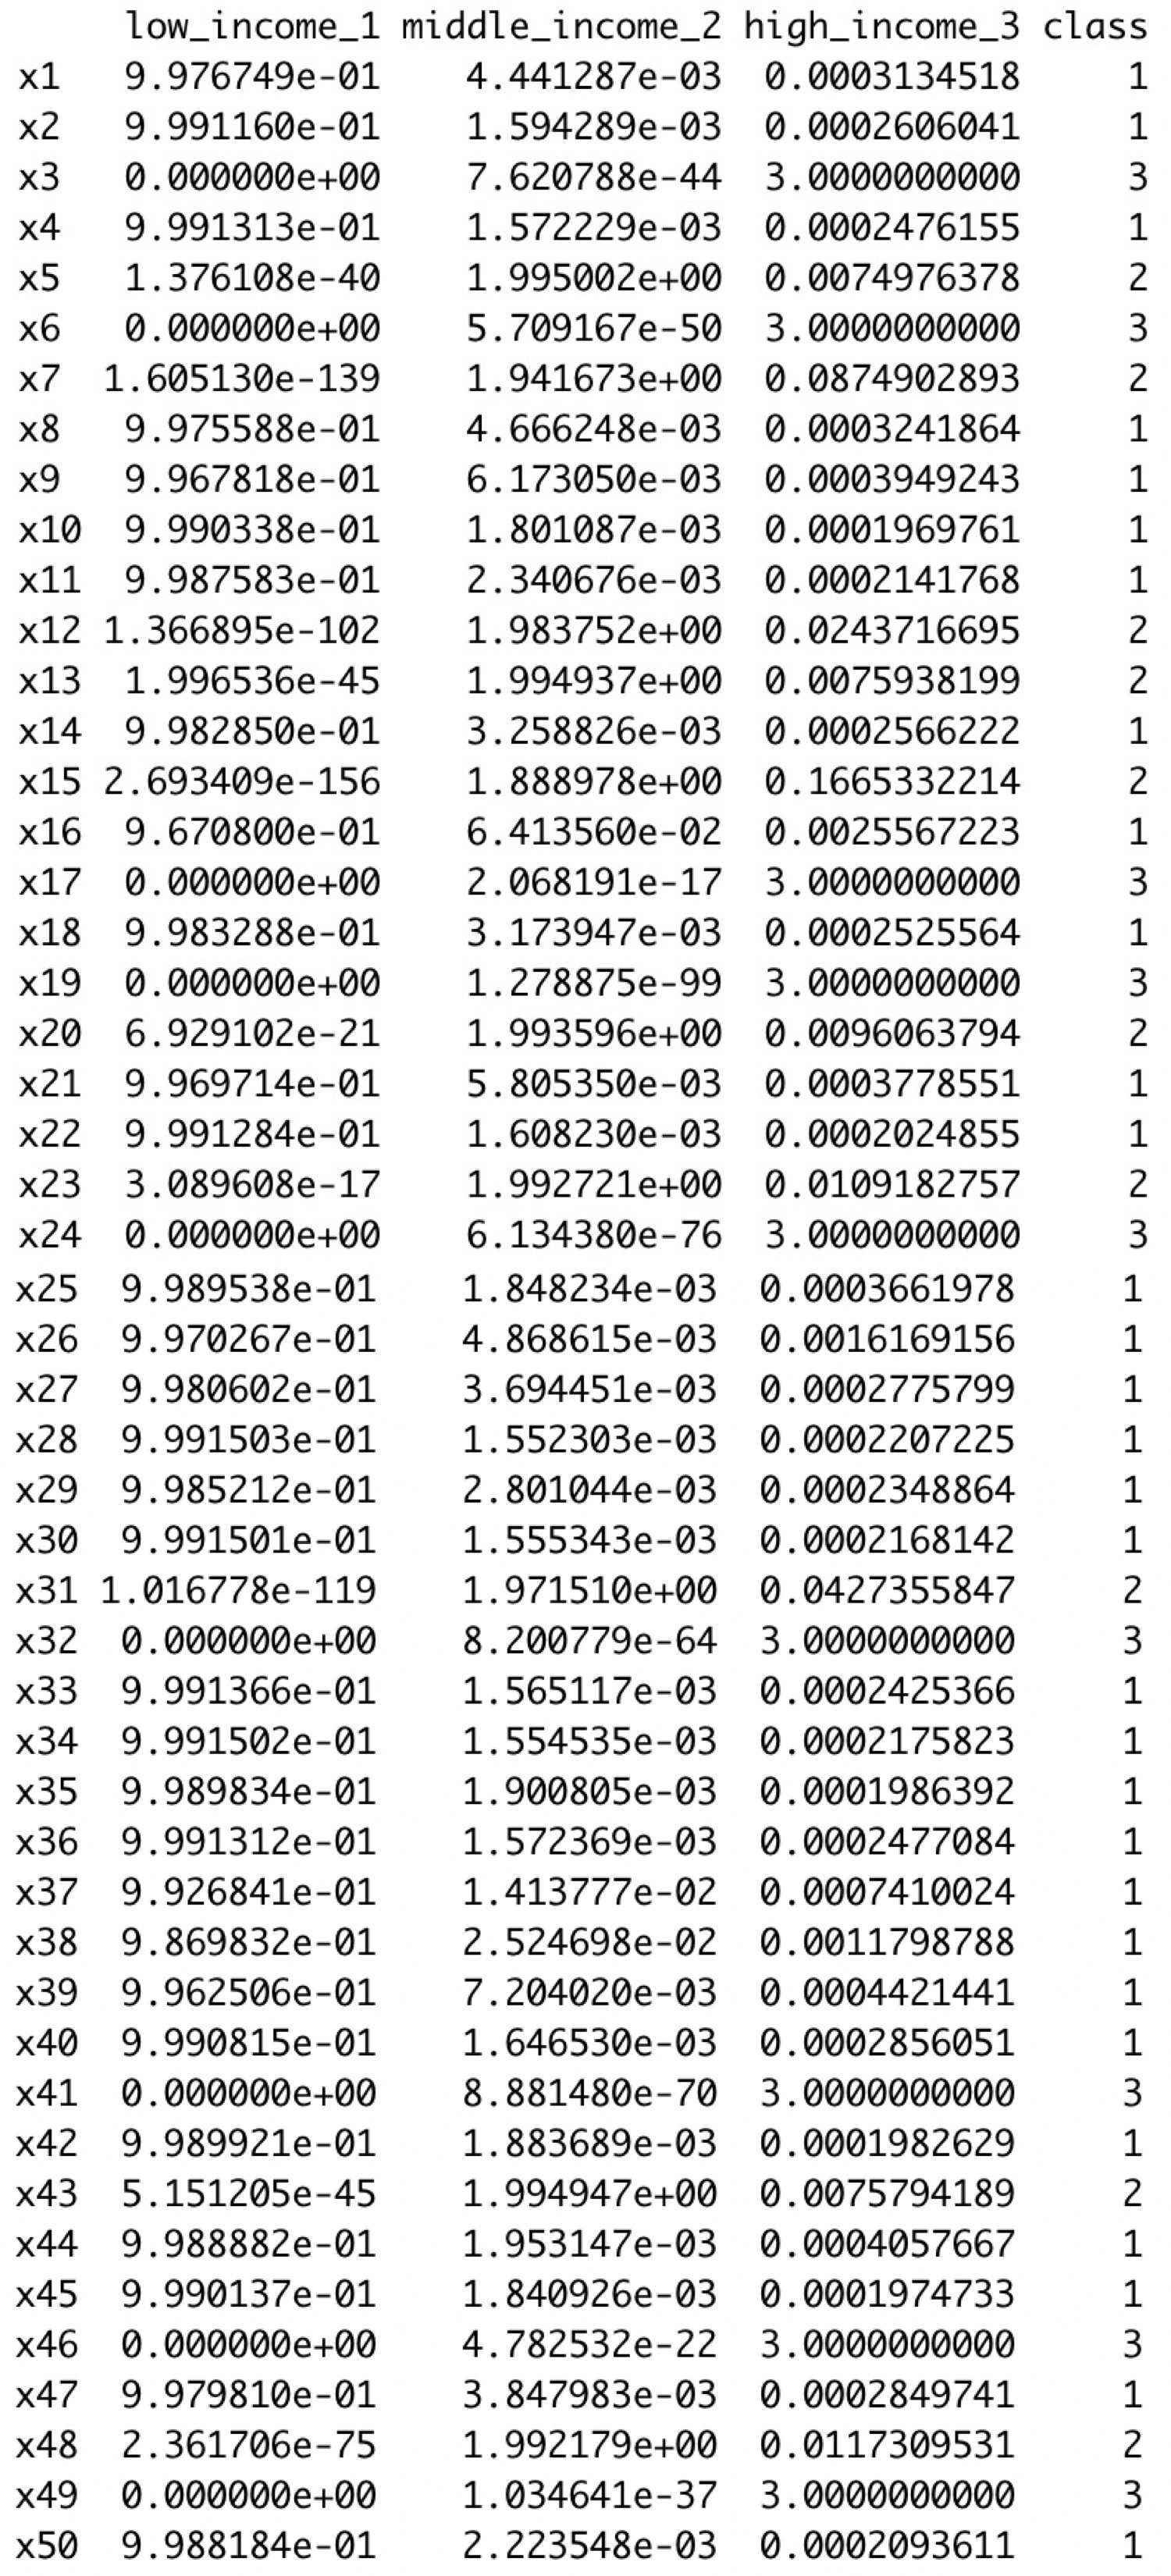
\includegraphics[width=0.6\textwidth]{result.JPG}
    \caption{Classification of first 50 individuals}
\end{figure}
}
\end{document}